%%
%  ******************************************************************************
%  * #file    Szablon_raportu_EN_Latex.tex
%  * #author  Adrian Wójcik   adrian.wojcik(at)put.poznan.pl
%  *          
%  * #commit  Patryk Kościk   koscikpatryk(at)gmail.com
%  *          Modified the template for Projekt przejsciowy purposes          
%  *          
%  *
%  * #commit  Patryk Kościk   koscikpatryk(at)gmail.com
%  *          Zupełnie przewrócono na łeb formatke po taktycznym wyjasnieniu          
%  *          
%  * #version 1.1
%  * #date    09-Mar-2022
%  * #brief   PROJPRZEJ
%  *
%  ******************************************************************************
%%  
\documentclass[11pt, a4paper]{article}

\usepackage{SM_template}

% Wypełnijcie te dyrektywy zgodnie z waszym tematem
%
% \lab      -> NAZWA CZUJNIKA,          np.: 'DHT22'
% \comment  -> Króciutki opis co to,    np.: 'Cyfrowy czujnik temperatury'
% \author   -> Autor dokumentu          np.: Patryk Kościk
%
% Pamiętajcie o zmianie ścieżki w \addbibresourcue (!)

\lab{Moduł KY-028}
\comment{Moduł czujnika temperatury}
\author{Dawid Sobczak}
\addbibresource{bib/KY-028.bib}

%
% Początek dokumentu
%
\begin{document}

%
% Strona tytułowa
%
\mainpage{KY-028/zdj_modułu/ky-028_module.PNG}
\newpage

\section*{Opis elementu}
KY-028 to moduł czujnika temperatury, który jako element pomiarowy wykorzystuje termistor NTC w układzie dzielnika napięcia z rezystorem 10000 [$\Omega$]. Moduł zasilany napięciem od 3.7 do 5.0 V zapewnia pomiar temperatury w  zakresie od -55 do +125 stopni Celsjusza oraz umożliwia manualną konfigurację zadanego progu temperatury, po którego przekroczeniu moduł wysyła informację w postaci zapalonej LED oraz stanu wysokiego na jednym z pinów.

\vspace{0.5cm}
W module wykorzystano termistor NTC, czyli rezystor o zmiennej pod wpływem temperatury rezystancji, gdzie skrót NTC oznacza, że wartość oporu spada wraz ze wzrostem temperatury. 
%%%%%%%%%%%%%%%%%%%%%%%%%  TWO IMAGES SIDE BY SIDE  %%%%%%%%%%%%%%%%%%%%%%%%%%%%%
\vspace{0.25cm}
\begin{figure}[h]
\centering
%%%%%%%%%%%%%%%%%%%%%%%%%%%%%%%%%%%%%%%%%%%%%%%%%%%%%%%%%%%%%%%%%%%%%%%%%%%%%%%%%
\begin{subfigure}{.5\textwidth}
\centering
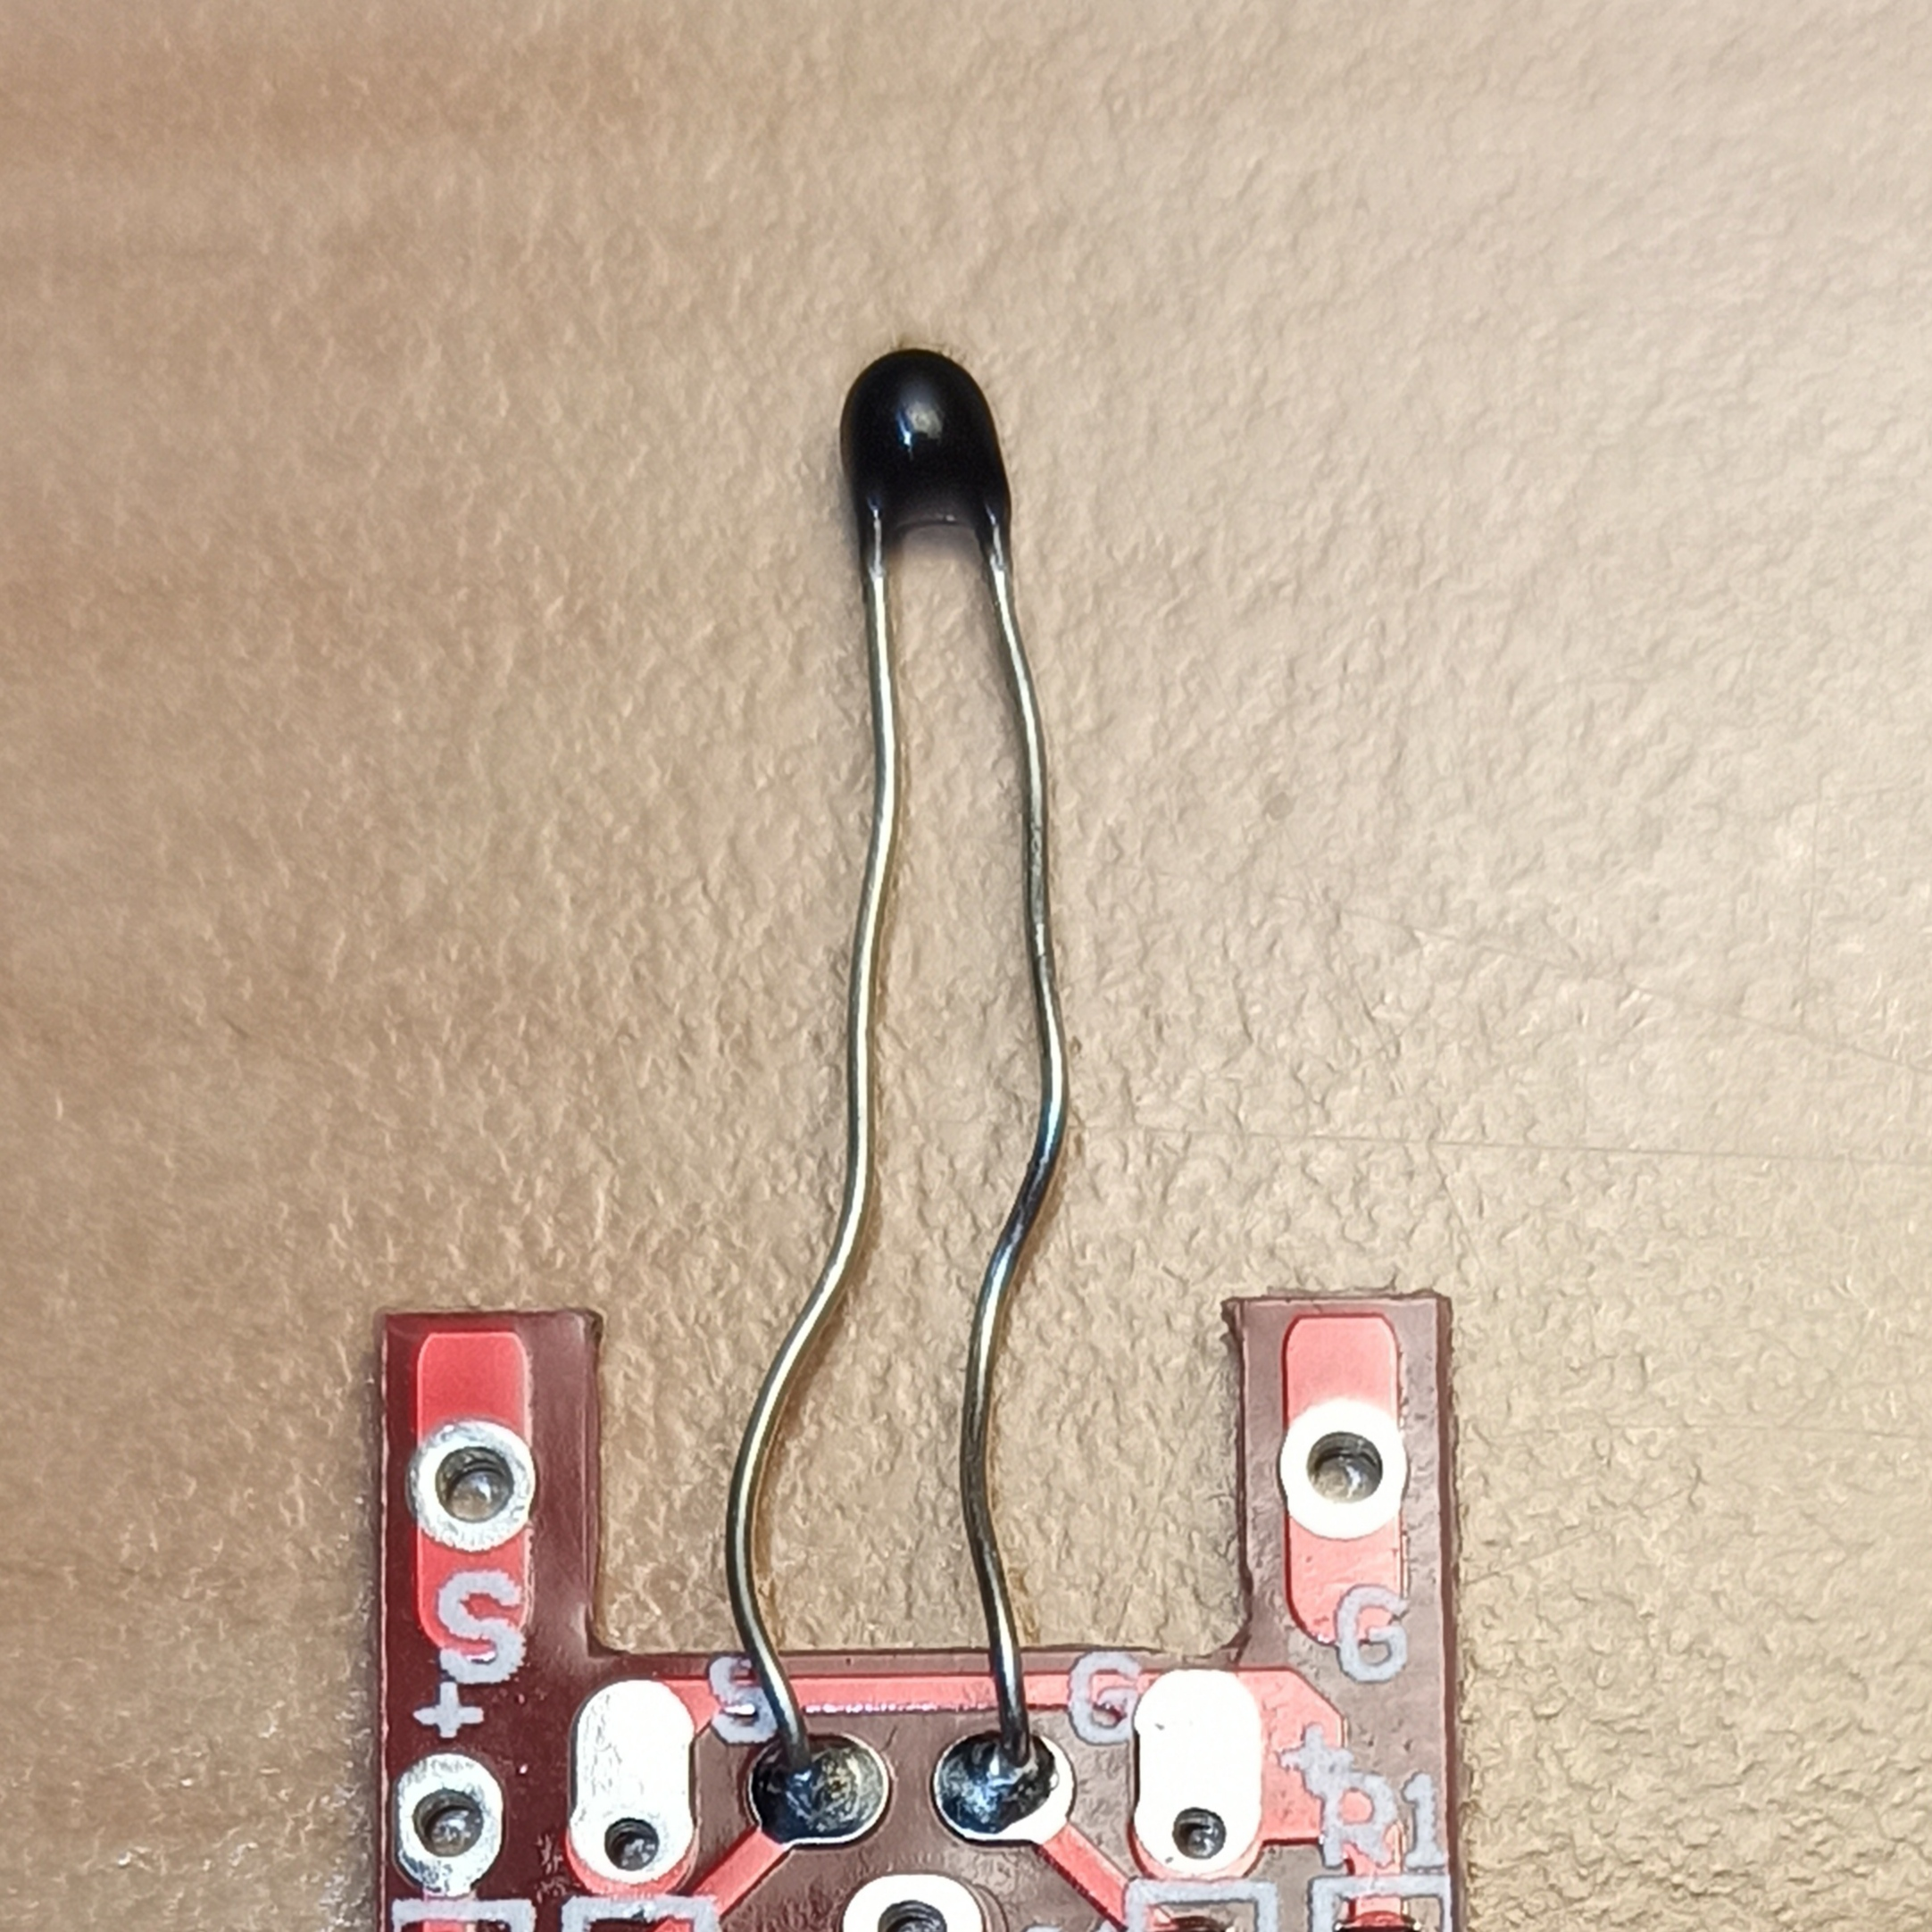
\includegraphics[width=.5\linewidth]{fig/KY-028/zdj_modułu/termistorNTC.jpg}
\caption{Termistor NTC w module KY-028}
\label{fig:_zdjecie_elementu}
\end{subfigure}%
%%%%%%%%%%%%%%%%%%%%%%%%%%%%%%%%%%%%%%%%%%%%%%%%%%%%%%%%%%%%%%%%%%%%%%%%%%%%%%%%%
\begin{subfigure}{.5\textwidth}
\centering
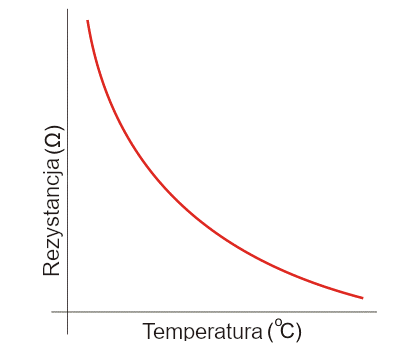
\includegraphics[width=.6\linewidth]{fig/KY-028/działanie_ukladu/ntc_charakterystyka.png}
\caption{Charakterystyka termistora NTC}
\label{fig:_zasada_dzialania_elementu}
\end{subfigure}
%%%%%%%%%%%%%%%%%%%%%%%%%%%%%%%%%%%%%%%%%%%%%%%%%%%%%%%%%%%%%%%%%%%%%%%%%%%%%%%%%
% \caption{PODPIS}
\label{fig:element}
\end{figure}
\vspace{0.25cm}
%%%%%%%%%%%%%%%%%%%%%%%%%  TWO IMAGES SIDE BY SIDE  %%%%%%%%%%%%%%%%%%%%%%%%%%%%%
% \subsection{Opis modułu} REPLACE SUBSECTION WITH 1CM VSPACE
\vspace{0.75cm}
%%%%%%%%%%%%%%%%%%%%%%%%%  TWO IMAGES SIDE BY SIDE  %%%%%%%%%%%%%%%%%%%%%%%%%%%%%
\begin{figure}[h]
\centering
%%%%%%%%%%%%%%%%%%%%%%%%%%%%%%%%%%%%%%%%%%%%%%%%%%%%%%%%%%%%%%%%%%%%%%%%%%%%%%%%%
\begin{subfigure}{.5\textwidth}
\centering
\includegraphics[width=.5\linewidth]{fig/KY-028/zdj_modułu/ky-028_photo.jpg}
\caption{Zdjęcie modułu KY-028}
\label{fig:_zdjecie_modulu}
\end{subfigure}%
%%%%%%%%%%%%%%%%%%%%%%%%%%%%%%%%%%%%%%%%%%%%%%%%%%%%%%%%%%%%%%%%%%%%%%%%%%%%%%%%%
\begin{subfigure}{.5\textwidth}
\centering
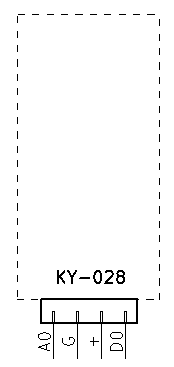
\includegraphics[width=.25\linewidth]{fig/KY-028/zdj_modułu/ky-028_pinout.PNG}
\caption{Wyprowadzenia modułu KY-028}
\label{fig:_schemat_modulu}
\end{subfigure}
%%%%%%%%%%%%%%%%%%%%%%%%%%%%%%%%%%%%%%%%%%%%%%%%%%%%%%%%%%%%%%%%%%%%%%%%%%%%%%%%%
\label{fig:modul}
\end{figure}
\vspace{0.5cm}
%%%%%%%%%%%%%%%%%%%%%%%%%  TWO IMAGES SIDE BY SIDE  %%%%%%%%%%%%%%%%%%%%%%%%%%%%%

Dodatkowo ważną cechą jest fakt, że zależność pomiędzy temperaturą a rezystancją termistora NTC jest nieliniowa.

\vspace{0.5cm}
Określona jest ona wzorem (\ref{eqn:temp_ress}):
%%%%%%%%%%%%%%%%%%%%%%%%%%% NTC THERMISTOR EQUATION
\begin{equation}
    R_T = R_0 \cdot e^{\beta(\frac{1}{T}-\frac{1}{T_0})}
    \label{eqn:temp_ress}
\end{equation}
Gdzie:
\begin{itemize}
    \item $R_T$ to rezystancja przy temperaturze $T$ (K*)
    \item $R_0$ to rezystancja przy temperaturze $T_0$ (K)
    \item $T_0$ to temperatura odniesienia (typowo 25 stopni C)
    \item $\beta$ to stała, zależna od matriału (typowo wartość nominalan to 4000)
\end{itemize}
*K - stopnie Kelvina
\newpage
\begin{figure}[h]
    \centering
    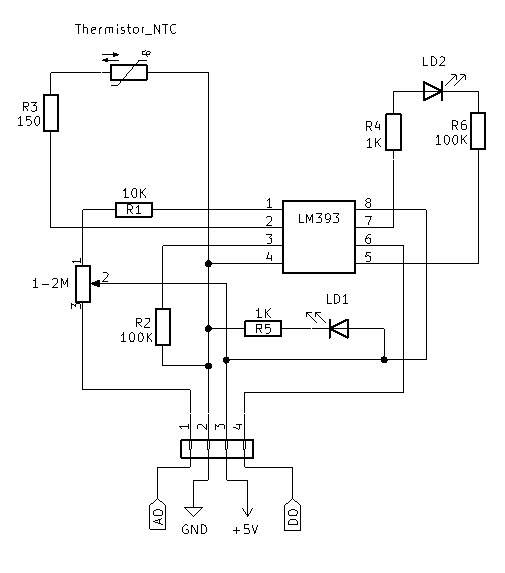
\includegraphics[width=0.8\textwidth]{fig/KY-028/zasada_dzialania/schemat_ky028.PNG}
    \caption{Kompletny schemat modułu KY-028}
    \label{fig:polaczenie_ukladu}
\end{figure}
\newpage
\section{Użycie modułu}
Najprostszym użyciem modułu jest zmierzenie wartości napięcia za pomocą multimetru bądź oscyloskopu. Moduł KY-028 zwraca na pinie 1 o oznaczeniu $A0$ wartość napięcia z dzielnika napięcia, który tworzy termistor NTC w układzie z rezystancją 10000 [$\Omega$].

\vspace{0.5cm}
% TUTAJ FOTY ODNOSNIE TEGO
%%%%%%%%%%%%%%%%%%%%%%%%%  TWO IMAGES SIDE BY SIDE  %%%%%%%%%%%%%%%%%%%%%%%%%%%%%
\vspace{0.25cm}
\begin{figure}[h]
\centering
%%%%%%%%%%%%%%%%%%%%%%%%%%%%%%%%%%%%%%%%%%%%%%%%%%%%%%%%%%%%%%%%%%%%%%%%%%%%%%%%%
\begin{subfigure}{.5\textwidth}
\centering
\includegraphics[width=.9\linewidth]{fig/KY-028/działanie_ukladu/22.jpg}
\caption{\centering Wskazanie multimetru dla temperatury pokojowej (około 22 stopnie Celsjusza)}
\label{fig:_uklad_woltomierz_otw}
\end{subfigure}%
%%%%%%%%%%%%%%%%%%%%%%%%%%%%%%%%%%%%%%%%%%%%%%%%%%%%%%%%%%%%%%%%%%%%%%%%%%%%%%%%%
\begin{subfigure}{.5\textwidth}
\centering
\includegraphics[width=.9\linewidth]{fig/KY-028/działanie_ukladu/ogrzane.jpg}
\caption{\centering Wskazanie multimetru przy lekkim ogrzaniu otoczenia termistora}
\label{fig:_uklad_woltomierz_zmk}
\end{subfigure}
%%%%%%%%%%%%%%%%%%%%%%%%%%%%%%%%%%%%%%%%%%%%%%%%%%%%%%%%%%%%%%%%%%%%%%%%%%%%%%%%%
% \caption{PODPIS}
\label{fig:woltomierz}
\end{figure}
\vspace{0.25cm}
%%%%%%%%%%%%%%%%%%%%%%%%%  TWO IMAGES SIDE BY SIDE  %%%%%%%%%%%%%%%%%%%%%%%%%%%%%
\vspace{0.5cm}
Aplikacja modułu wymaga połączenie mikrokontrolera z modułem w sposób opisany w tabeli (\ref{tab:tab1}) znajdującej się poniżej.

\vspace{0.5cm}
\begin{table}[h!]
    \centering
    \begin{tabular}{|c|c|c|c|} 
        \hline
        \multicolumn{2}{|c|}{NUCELO-F746ZG} & \multicolumn{2}{c|}{KY-028}  \\ 
        \hline
        Etykieta & Port i numer pinu       & Nr pinu & Etykieta           \\ 
        \hline
        D32      & PA0                     & 1       & A0             
        \\
        \hline
        GND      & -                    & 2       & G           
        \\
        \hline
        +5V      & -                      & 3       & +              \\
        \hline
        D43      & PC8                       & 4       & D0              \\
        \hline
    \end{tabular}
    \caption{Połącznie pomiędzy modułem i mikrokontrolerem}
    \label{tab:tab1}
\end{table}

Dodatkowe schematy połączeń i konfiguracja
mikrokontrolera została opisana w sekcji \texttt{Suplement \#1}. Zawiera tam się również kod języka
C + HAL, pozwalający na obsługę modułu.

\newpage
\begin{figure}[h]
    \centering
    \includegraphics[width=0.55\textwidth]{fig/KY-028/polaczenie_modulu/connection_zdj.jpg}
    \caption{Połączenie układu}
    \label{fig:polaczenie_ukladu}
\end{figure}
\begin{figure}[h]
    \centering
    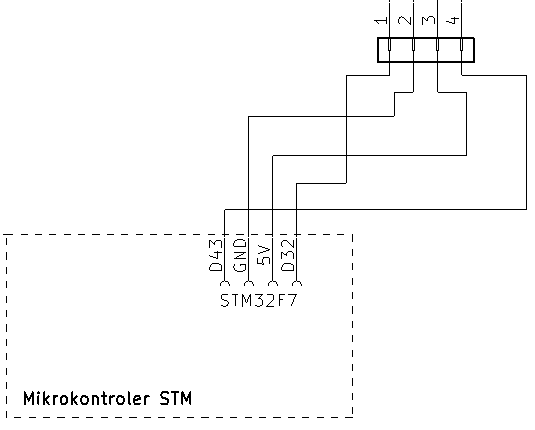
\includegraphics[width=0.5\textwidth]{fig/KY-028/polaczenie_modulu/stm_f7_ky_028_connection.PNG}
    \caption{Schemat połączenia układu}
    \label{fig:schemat_polaczenie_ukladu}
\end{figure}


Więcej informacji na temat kodu i oprogramowania zawarte jest w \texttt{Suplement \#1}.

\vspace{0.5cm}
Dodatkowo działanie układu przedstawiono na załączonym w \texttt{\cite{yt1}} oraz w \texttt{\cite{yt2}} materiale wideo. Materiały zawierają kalibrację modułu oraz przykładowy pomiar wartości temperatury. 

\newpage
\printbibliography[heading=bibintoc]

\end{document}